\documentclass{article} % For LaTeX2e
\usepackage{amsthm}
\usepackage{amssymb}
\usepackage{amsmath}
\usepackage{bibentry}
\usepackage{caption}
\usepackage{filecontents}
\usepackage{hyperref}
\usepackage{listings}
\usepackage{natbib}
\usepackage{pgfplots}
\usepackage{tikz}
\usetikzlibrary{bayesnet}
\usepackage{wrapfig}
\usepackage{xstring}
\usepackage{url}

\usepackage{nips14submit_e}
\usepackage{times}


\title{Title}

\author{
Tal Friedman \\
\texttt{talf301@gmail.com} \\
\And
Erin Grant \\
\texttt{erin.grant@mail.utoronto.ca}
}


\newcommand{\fix}{\marginpar{FIX}}
\newcommand{\new}{\marginpar{NEW}}
\newcommand{\argmax}{\operatornamewithlimits{argmax}}

% Reference label commands
\newcommand{\Table}[1]{Table~\ref{#1}}
\newcommand{\Algorithm}[1]{Algorithm~\ref{#1}}
\newcommand{\Section}[1]{Section~\ref{#1}}
\newcommand{\Example}[1]{\ref{#1}}
\newcommand{\Figure}[1]{Figure~\ref{#1}}
\newcommand{\Equation}[1]{Eqn.~(\ref{#1})}
\newcommand{\Page}[1]{page~\pageref{#1}}


%% colour definitions
\definecolor{pink}{HTML}{F67088}
\definecolor{orange}{HTML}{CE8F31}
\definecolor{green}{HTML}{32B165}
\definecolor{blue}{HTML}{38A7D0}
\definecolor{purple}{HTML}{A38CF4}


%% tikz definitions

% bayes net nodes
\tikzstyle{item on} = [draw, circle, fill=blue!50, text centered, minimum size=3em]
\tikzstyle{item off} = [draw, circle, fill=blue!25, text centered, minimum size=3em] 
\tikzstyle{hidden on} = [draw, circle, fill=orange!50, text centered, minimum size=3em]
\tikzstyle{hidden off} = [draw, circle, fill=orange!25, text centered, minimum size=3em] 
\tikzstyle{query on} = [draw, circle, fill=purple!50, text centered, minimum size=3em]
\tikzstyle{query off} = [draw, circle, fill=purple!25, text centered, minimum size=3em] 

% ontology nodes
\tikzstyle{disease} = [draw, rectangle, rounded corners, fill=blue!25, text centered, align=center]
\tikzstyle{phenotype} = [draw, rectangle, rounded corners, fill=purple!25, text centered, align=center]

% algorithm style
\lstnewenvironment{algorithm}[1][] %defines the algorithm listing environment
{   
    \lstset{
        frame=tb,
        commentstyle=\itshape,
        numbers=left, 
        numberstyle=\tiny,
        keywordstyle=\color{black}\bfseries,
        keywords={,input, output, return, in, if, else, foreach, while, },
        xleftmargin=.04\textwidth,
        mathescape=true,
    }
}
{}


%\nipsfinalcopy % Uncomment for camera-ready version


\begin{document}

%\nobibliography*

\maketitle


\begin{abstract}

    Blah blah blah.

\end{abstract}


\section{Introduction}
\label{sec:intro}

[TODO: introduce disease diagnosis in general, reference QR network or something like that]
Computer assisted diagnosis is a useful and desirable tool that has been challenging the AI community for many years. Jaakkola et Al. \cite{qmrdt} introduced the QMR-DT network, a major example  of a probabilistic graphical model built on expert knowledge used for CAD. 
CAD is particularly useful in the realm of rare genetic diseases, where clinical geneticists will often be tasked with diagnosing patients with disorders they may only see a couple of times in their careers. In this regard, having a tool which can make some reasonable suggestions for diagnoses a clinician may have never seen before is invaluable. \\
In order for a CAD system to be feasible, one requires either a very large training set of diagnosed patients, or some expert information relating disorders and symptoms. Clearly, the first option is not a possibility in our domain, but the Human Phenotype Ontology (HPO) \cite{kohler2014hpo} and Online Mendelian Inheritance in Man (OMIM) \cite{omim} together introduce respectively a powerful, standardized dictionary for describing human conditions as well as disorders and their associated symptoms.

% TODO: emphasise that we are talking about rare genetic diseases and not other types of diseases
\section{Previous Work}
\label{sec:lit-rev}

\cite{bauer2012bayesian} introduce Bayesian inference into a query system.

Their network comprises three layers of Boolean variables: an {\it item} layer
of diseases, a {\it hidden} layer of phenotypic features, and a {\it query}
layer of phenotypic features.
%
Each node in the query layer corresponds to exactly one node in the hidden
layer.

The causal relationship between a disease and its potential symptoms is modelled
as a set of directed edges from a disease node in the {\it item} layer to a
subset of the phenotypic nodes in the {\it hidden} layer.

The {\it hidden} layer is then connected to the {\it query} layer in a
one-to-one fashion by a directed edge from a phenotype node in the {\it hidden}
layer to its correspondent in the {\it query} layer.

Furthermore, there are within-layer connections to model the ontology of
symptoms given by the Human Phenotype Ontology (HPO) \cite{kohler2014hpo}.

Within the {\it hidden} layer, there is a directed edge from node $H_i$ to $H_j$
if the annotation of the phenotype $H_i$ implies that the phenotype $H_j$ is
also present.

Such an edge is present in the network if the phenotype $H_i$ is a child of
phenotype $H_j$ in the HPO; these edges serve the purpose of encoding the {\it
annotation propagation rule}: if an item $j$ is annotated to term $i$ then it is
implicitly annotated to all ancestors of $i$.

In the case that the edge is present, in the {\it query} layer, there is a
directed edge from phenotype $Q_j$ to phenotype $Q_i$ (i.e., an edge in the
inverse direction of the edge $H_i \to H_j$).

%See \Figure{fig:bauer-net}.
%
%\begin{wrapfigure}{r}{0.5\textwidth}
%    \label{fig:bauer-net}
%\end{wrapfigure}

\subsection{Network construction}

Let $M$ represent the number of terms in the ontology, and let $N$ represent the
number of diseases.

Let 
$\{I_i\}_{i=1}^{N}, 
\{H_j\}_{j=1}^{M}$ and 
$\{Q_k\}_{k=1}^{M}$ represent the nodes in the {\it item}, {\it hidden} and {\it
query} layers, respectively.

Indices of phenotypic nodes in this network correspond to indices of terms in
the HPO;
%
i.e., $H_i$ and $Q_i$ together correspond to the $i$th node in the ontology.
%
Identify parent-child relations from the ontology in the following manner:
%
let pa$(i) = \{\text{pa}(i)_1, \hdots, \text{pa}(i)_J\}$ denote the $J$ indices
of the direct parents of term $i$ in the ontology, 
%
and similarly let chi$(i) = \{\text{chi}(i)_1, \hdots, \text{chi}(i)_K\}$ to
denote the $K$ indices of the direct children of term $i$ in the ontology.

Furthermore, indices of disease nodes in the network correspond to indices of
diseases that are annotated by terms in the HPO.
%
Identify the annotations for a disease as follows: let ea$(j) =
\{\text{ea}(j)_1, \hdots, \text{ea}(j)_L\}$ denote the indices of the $L$ terms
for which the $j$th disease is explicitly annotated.

The local probability distributions for the hidden nodes can then be written as
%
\begin{align}
    P \left(H_i = 1 \mid I_{\text{ea}(i)}, \bigvee H_{\text{chi}(i)}\right)
    &= \left(
        1 - \prod_{j=\text{ea}(i)_1}^{\text{ea}(i)_L}
        \left(1 - I_j \, f_{ji}\right)
    \right)
    ^{1 - \bigvee H_{\text{chi}(i)}}
    \label{eq:lpdhids}
\end{align}
%
where $\bigvee$ represents the logical disjunction, and $f_{ji}$ represents the
empirical frequency of the occurrence of phenotype $i$ with disease $j$.
%
This formulation captures the annotation propagation rule within the hidden,
since it evaluates to $1$ if $\bigvee H_{\text{chi}(i)} = 1$; that is, if any
child annotations are active.
%
As well, it captures that the hidden node is inactive with probability 1 if all
diseases are inactive (i.e., $I_i = 0, \forall i$), and otherwise the
probabillity of activity in the hidden state is a function of the emprical
association of disease and symptom.

The local probability distribution for the query nodes, given the states of
$H_i$ and $Q_{\text{pa}(i)}$, can be written as
%
\begin{align*}
    \begin{aligned}[c]
        P\left(Q_i = 0 \mid H_i = 1, \bigwedge Q_{\text{pa}(i)} = 0\right) &= 1 \\
        P\left(Q_i = 1 \mid H_i = 1, \bigwedge Q_{\text{pa}(i)} = 0\right) &= 0 \\
        P\left(Q_i = 0 \mid H_i = 1, \bigwedge Q_{\text{pa}(i)} = 1\right) &= \beta \\
        P\left(Q_i = 1 \mid H_i = 1, \bigwedge Q_{\text{pa}(i)} = 1\right) &= 1 - \beta \\
    \end{aligned}
    \qquad
    \begin{aligned}[c]
        P\left(Q_i = 0 \mid H_i = 0, \bigwedge Q_{\text{pa}(i)} = 0\right) &= 1 \\
        P\left(Q_i = 1 \mid H_i = 0, \bigwedge Q_{\text{pa}(i)} = 0\right) &= 0 \\
        P\left(Q_i = 0 \mid H_i = 0, \bigwedge Q_{\text{pa}(i)} = 1\right) &= 1 - \alpha \\
        P\left(Q_i = 1 \mid H_i = 0, \bigwedge Q_{\text{pa}(i)} = 1\right) &= \alpha
    \end{aligned}
\end{align*}
%
where $\bigwedge$ represents the logical conjunction, $\beta$ represents the
probability of a false negative (i.e., $H_i = 1$ but $Q_i = 0$), and $\alpha$
represents the probability of a false positive (i.e., $Q_i = 1$ but $H_i = 0)$.

Now, defining a variable $m_{xyz\mid QH}$ by
%
\begin{align*}
    m_{xyz\mid QH} 
    &= \left| 
        \left\{k \mid
        \left(
            Q_k = x 
        \right) \wedge  \left(
            H_k = y
        \right) \wedge  \left(
            \bigwedge Q_{\text{pa}(k)} = z
        \right)
        \right\}
    \right|,
\end{align*}
%
the joint probability of the query nodes $Q_i$ may be written as
%
\begin{align*}
    \prod_{i=1}^M P\left(Q_i \mid H_i, \bigwedge Q_{\text{pa}(i)}\right)
    &=  \beta^{\,m_{011\mid QH}}
    \;(1 - \beta)^{m_{111\mid QH}}
    \;\alpha^{m_{001\mid QH}}
    \;(1 - \alpha)^{m_{101\mid QH}},
\end{align*}
under the assumption that the invalid configurations $m_{110\mid QH}$ and
$m_{100\mid QH}$ occur with probability zero,
%
and using the simplification that the configurations $m_{010\mid QH}$ and
$m_{000\mid QH}$ have probability one.

The joint probability distribution over the network is then realised as
%
\begin{align}
    &P(I_1, \hdots, I_N, H_1, \hdots, H_M, Q_1, \hdots, Q_M) \nonumber\\
    &=  P(I_1, \hdots, I_N) 
    \; \prod_{i=1}^M P\left(H_i \mid \bigvee I_{\text{ea}(i)}, \bigvee H_{\text{chi}(i)}\right)
    \; P\left(Q_i \mid H_i, \bigwedge Q_{\text{pa}(i)}\right). \label{eq:joint}
\end{align}

\subsection{Inference}

The marginal probability of a configuration of the disease nodes $I_1, \hdots,
I_N$ in the item layer, given some phenotypic evidence $Q_1, \hdots, Q_M$, is
given by marginalising over $\vec{H}$ as
%
\begin{align*}
    P(I_1, \hdots, I_n \mid Q_1, \hdots, Q_M)
    &= \frac{\sum_{\vec{H}} P(I_1, \hdots, I_n, H_1, \hdots, H_M, Q_1, \hdots, Q_M)}{P(Q)} \\
    &= \frac{\sum_{\vec{H} \in \{0, 1\}^M} P(I_1, \hdots, I_n, H_1, \hdots, H_M, Q_1, \hdots, Q_M)}{P(Q)} \\
\end{align*}

The goal of this model is to find the configuration of diseases with highest
posterior probability, given some phenotypic evidence.
%
This is a MAP inference problem, and so may be solved by maximising the product
of the likelihood and the prior; i.e., the solution is given by
%
\begin{align}
    &\argmax_{(I_1, \hdots, I_N)} \;
    P(I_1, \hdots, I_N \mid Q_1, \hdots, Q_M) \nonumber\\
    &= \argmax_{(I_1, \hdots, I_N)} \;
    \frac{P(Q_1, \hdots, Q_M \mid I_1, \hdots, I_N )\; P(I_1, \hdots, I_N)}{P(Q)} \nonumber\\
    &= \argmax_{(I_1, \hdots, I_N)} \;
    P(Q_1, \hdots, Q_M \mid I_1, \hdots, I_N )\; P(I_1, \hdots, I_N) \nonumber\\
    &= \argmax_{(I_1, \hdots, I_N)} \;
    P(I_1, \hdots, I_N)
    \;\sum_{\vec{H} \in \{0, 1\}^M} \; \prod_{i=1}^M \; P\left(H_i \mid \bigvee I_{\text{ea}(i)}, \bigvee H_{\text{chi}(i)}\right)
    \; P\left(Q_i \mid H_i, \bigwedge Q_{\text{pa}(i)}\right).\label{eq:mapinf}
\end{align}

\subsection{Complexity restrictions}

The computation in \Equation{eq:mapinf} is intractable, since 
there are $2^N$ configurations of the item nodes over which to maximise the
posterior, and there are $2^M$ configurations of the hidden nodes $H_1, \hdots,
H_M$ over which to marginalise.
%
Bauer et al.\ make two simplifications to make inference tractable; we describe
them in \Section{subsubsec:odc} and \Section{subsubsec:kleast}.

\subsubsection{One-disease constraint}
\label{subsubsec:odc}

To avoid maximising over the $2^N$ configurations of the item nodes, Bauer et al.\
impose the constraint
%
\begin{align}
    \sum_{i=1}^N I_i = 1. \label{eq:onehot}
\end{align}
%
\Equation{eq:onehot} enforces the restriction that only one disease node may be
active given any query, and so the maximum is taken over $N$ one-hot
configurations for the MAP estimate.
%
This is equivalent to assuming that a patient can have only a single disease;
%
since this is a diagnosis system for rare genetic diseases, this is a reasonable
assumption.
%
Therefore, we adopt the one-disease constraint into all models that we describe
in \Section{sec:models}.

\subsubsection{$k$-least frequency annotations constraint}
\label{subsubsec:kleast}

To avoid marginalising over the $2^M$ configurations of the hidden nodes,
Bauer et al.\ simplify the local probability distribution of each hidden node
that is given by \Equation{eq:lpdhids}.
%
In particular, they restrict the number of frequency annotations $f_{ji}$, for
each disease node $I$, that are not exactly zero or exactly one, to the
annotations with the $k$ least frequency values.
%
\footnote{
    Bauer et al.\ use $k=10$ for their final experimental results.
}
%
This has the effect of enforcing all other hidden node likelihoods
to be either active or inactive with probability one,
conditional on a disease node $I$.
%
Therefore, to compute the sum over in $\vec{H} \in \{0, 1\}^M$ in
\Equation{eq:mapinf}, the model need only take into account the subset of
summands representing configurations in which the likelihood of all hidden nodes
with deterministic activity is one, since the remaining terms are zero.
%
This makes the marginalisation computationally tractable by restricting the
magnitude of the marginalisation.
%
In \Section{sec:models}, we describe models that either adopt or relax this
constraint.

\section{Objectives}
\label{sec:obj}

What are we trying to solve and how are we gonna do it?


Let $(Q_1, ..., Q_M)$ be query variables.
Let $I_1$ be a disease that is explicitly negatively annotated to $Q_1$.
Let $I_2$ be a disease that is not explicitly annotated to $Q_1$.
Let $I_3$ be a disease that is explicitly annotated to $Q_1$.

\begin{align*}
    P(Q_1 = 0, \hdots, Q_M \mid I_1) \\
    P(Q_1 = 1, \hdots, Q_M \mid I_3) \\
    P(Q_1 = 0, \hdots, Q_M \mid I_2) \\
    P(Q_1 = 1, \hdots, Q_M \mid I_2) \\
    P(Q_1 = 0, \hdots, Q_M \mid I_3) \\
    P(Q_1 = 1, \hdots, Q_M \mid I_1) 
\end{align*}
      
\section{Modifications}
\label{sec:models}

In this section we describe the various modifications to
the network structure and inference procedure made in order to incorporate the
desired functionality.
\footnote{
    Our code can be found at
    \url{https://github.com/talf301/boqa-negative}.
    We reimplemented the BOQA baseline codebase in Python, and manually coded all
    modifications described in this section.
}

\subsection{Modification to the network structure}
\label{subsec:modnetstruct}

Recall that in the BOQA network, the probability of activity in a hidden node is
realized as  
%
\begin{align}\label{eq:lpdhidden}
    P \left(H_i = 1 \mid I_{\text{ea}(i)}, \bigvee H_{\text{chi}(i)}\right)
    &= \left(
        1 - \prod_{j=\text{ea}(i)_1}^{\text{ea}(i)_L}
        \left(1 - I_j \, f_{ji}\right)
    \right)
    ^{1 - \bigvee H_{\text{chi}(i)}}
\end{align}
%
where $f_{ji}$ represents the empirical frequency of the occurrence of phenotype
$i$ with disease $j$.
%
Under this formulation, if disease $i$ is not annotated to phenotype $j$, 
and none of the children of $j$ are either (i.e., $\bigvee H_{\text{chi}(i)} = 0$),
then the probability of activity in the hidden layer is simply zero.
%
In other words, the likelihood of observing symptom $j$, given that the patient
has disease $i$, is zero.

However, since the symptom is not negatively annotated to the disease, we would
like the model instead to assign some likelihood to the occurrence of this event,
encoding the expectation that the symptom may occur together with the disease
by chance.
%
In particular, a likelihood of zero should be assigned only to those symptoms
that are negatively annotated to a disease.
%
We modify the local probability distribution in (\ref{eq:lpdhidden}) to capture
this specification as described in the following paragraphs.

Let $\text{pos}(i) = \{\text{pos}(i)_1, \hdots, \text{pos}(i)_S\}$, for each
$H_i$, index the $S$ diseases for which $H_i$ is explicitly positively
annotated and let $\text{neg}(i) = \{\text{neg}(i)_1, \hdots,
\text{neg}(i)_T\}$, the $T$ diseases for which $H_i$ is explicitly negatively
annotated.

Then if we let the probability of activity in a hidden node $H_j$ be given by
\begin{align}\label{eq:lpdhiddenmod1}
    &P\left(H_i = 1 \mid I_{\text{pos}(i)_1}, \hdots, I_{\text{pos}(i)_S},
    \bigvee I_{\text{neg}(i)}, \bigwedge H_{\text{chi}(i)}\right)\nonumber\\
        &= \left(
            1 - 
            \left(
                \prod_{j=\text{pos}(i)_1}^{\text{pos}(i)_S}
                \left(1 - I_j \, f_{ji}\right)
            \right) ^{1 - \bigvee I_{\text{neg}(i)}}
        \right)
        ^{1 - \bigvee H_{\text{chi}(i)}}
\end{align}
where if the empirical frequency is not available but the symptom $j$ is not
negatively annotated to disease $i$, then frequency $f_{ij}$ is set to some
small value, $p$.
%
\footnote{It should be noted that activity of a child annotation of a node
    $H_j$ entails activity in $H_j$ under the formulation in
    (\ref{eq:lpdhiddenmod1}), even if phenotype $j$ is negatively annotated
    to the disease of interest. However, this situation does not occur in the
    HPO, and so we need not treat special cases.
}

However, the result of this modification to the network is that exact inference
is now intractable, since marginalizing over all binary assignments to the
hidden nodes is exponential in the number of phenotypes,
as noted in \Section{subsubsec:kleast}. 
%
Furthermore, we may not apply the $k$-least frequencies restriction 
described in \Section{subsubsec:kleast}. 
to simplify the marginalization, since that would force some hidden nodes to
deterministically be inactive, conditional on activity in
some item node, even though the corresponding phenotypes may not be negatively
annotated to the active disease.
%
Therefore, we consider several methods to approximate computation of the
marginals, which we describe in the next sections.

\subsection{Modifications to the inference procedure}
\label{subsec:modinf}

We test two different methods of sampling to approximate inference in the
network.

\subsubsection{$p$-sampling}
\label{subsubsec:psampmodel}
%
As described for \Equation{eq:lpdhiddenmod1},
we assume that for each hidden node without an annotation (positive or negative), the frequency
has a fixed value of $p$. 
%
More details are given in \Section{subsubsec:psampexp}.

\subsubsection{Information-content sensitive $p$-sampling}
\label{subsubsec:icsampmodel}
%
Here, rather than using the value $p$ directly, we weight 
$p$ by the inverse information content of the phenotype
associated with the hidden node. \Equation{eq:infocontent} shows how
we compute the information content for each phenotype.
%
\begin{align}\label{eq:infocontent} 
    -\log_{2}\frac{\text{\# of times phenotype or its descendants is annotated to a disease}}{N},
\end{align}
where $N$ is the number of known diseases.
%
More details are given in \Section{subsubsec:icpsampexp}.

\section{Experiments}
\label{sec:exp}

\subsection{Artificial data generation}

The HPO \cite{kohler2014hpo} is a directed acyclic graph that depicts an
ontology of 10 476 phenotypes.
%
It specifies annotations for 6575 diseases, 471 of which possess negative
annotations.
%
In addition to using the ontology as expert information in the model
construction and inference procedures, we exploit it to generate patients
for testing.
%
\footnote{
    Rare genetic diseases is, true to its name, a domain in which there are few
    examples, so we have to generate more test data to fill the void.
}
%
We spawned 500 patients infected with diseases that
possess positive annotations but not necessarily negative annotations, and then
generated a further 471 patients each infected with a unique
negatively-annotated disease.

We generated and infected patients in the following manner:
%
\begin{enumerate}
    \item \label{enum:patgen1}
        For a given disease, we sampled each of the disease's annotated
        symptoms with probability equal to the empirical association of symptom
        and disease, as specified by the HPO.
    \item \label{enum:patgen2}
        To simulate noise in the patient queries, we added a number
        of unrelated symptoms to the patient query by sampling with uniform
        probability over all symptoms.
        \footnote{
            For all experimental results, we chose the number of noise symptoms
            to be half the number of symptoms generated in Step
            \ref{enum:patgen1}.
        }
    \item To simulate imprecision in the patient queries, for each symptom
        generated in Steps \ref{enum:patgen1} and \ref{enum:patgen2}, with some
        probability we replaced the symptom with one of its ancestors in the
        HPO.
        \footnote{
            Each symptom is replaced by another symptom chosen uniformly from a
            set containing all ancestors of the symptom and the symptom itself.
            In this way, there is some small probability that the symptom is
            retained, and thus the query is made no less precise.
        }
\end{enumerate}
%
We will refer to the data generated in this way as the {\it artificial patient
data}.

In addition to this artificially generated data, we tested all models
on 101 patient queries obtained from real-life clinician-patient
encounters, which we refer to as the {\it naturalistic patient data}.
%
\footnote{
    We take the naturalistic patients data from the PhenoTips patients
    repository \cite{phenotips}.
    The data is not publicly available.
}




\section{Results}
\label{sec:res}

Did we fail? \\
Yes!
\section{Discussion}
\label{sec:dis}

Discuss important things.
\section{Conclusion}
\label{sec:conc}

Draw groundbreaking conclusions.


\newpage
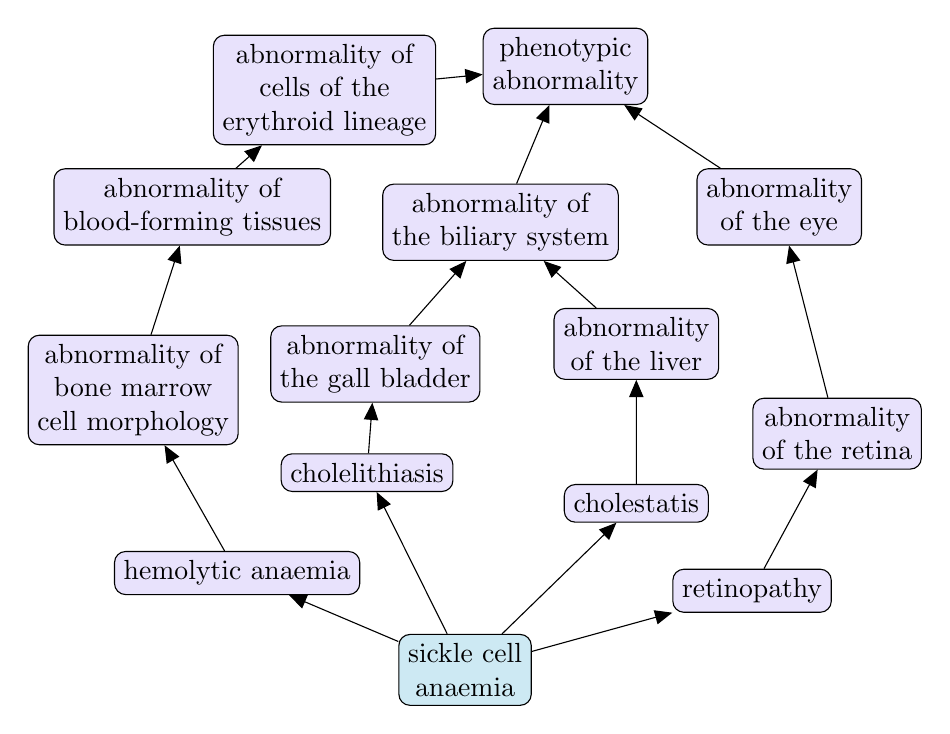
\begin{tikzpicture}[scale=0.15]
    \draw (39.9,-54.6) node[disease] (A) {sickle cell \\ anaemia};
    \draw (64.2,-47.9) node[phenotype] (B) {retinopathy};
    \draw (71.4,-34.6) node[phenotype] (C) {abnormality \\ of the retina};
    \draw (66.5,-15.4) node[phenotype] (D) {abnormality \\ of the eye};
    \draw (48.4,-3.5)  node[phenotype] (E) {phenotypic \\ abnormality};
    \draw (54.4,-40.5) node[phenotype] (F) {cholestatis};
    \draw (54.4,-27)   node[phenotype] (G) {abnormality \\ of the liver};
    \draw (42.9,-16.7) node[phenotype] (H) {abnormality of \\ the biliary system};
    \draw (31.6,-37.9) node[phenotype] (I) {cholelithiasis};
    \draw (32.3,-28.7) node[phenotype] (J) {abnormality of \\ the gall bladder};
    \draw (20.6,-46.4) node[phenotype] (K) {hemolytic anaemia};
    \draw (11.8,-30.9) node[phenotype] (L) {abnormality of \\ bone marrow \\ cell morphology};
    \draw (16.8,-15.4) node[phenotype] (M) {abnormality of \\ blood-forming tissues};
    \draw (28,-5.5)    node[phenotype] (N) {abnormality of \\ cells of the \\ erythroid lineage};
    \edge {A} {B};
    \edge {A} {F};
    \edge {A} {I};
    \edge {A} {K};
    \edge {B} {C};
    \edge {C} {D};
    \edge {D} {E};
    \edge {F} {G};
    \edge {G} {H};
    \edge {I} {J};
    \edge {J} {H};
    \edge {K} {L};
    \edge {L} {M};
    \edge {M} {N};
    \edge {N} {E};
    \edge {H} {E};
\end{tikzpicture}

\newcommand{\itemlayer}{$I_1$/A, $I_2$/B}
\newcommand{\hiddenquerylayers}{$H_1$/C/$Q_1$/J, $H_2$/D/$Q_2$/K, $H_3$/E/$Q_3$/L, $H_4$/F/$Q_4$/M, $H_5$/G/$Q_5$/N, $H_6$/H/$Q_6$/O, $H_7$/I/$Q_7$/P}

\begin{figure}[h]
    \begin{tikzpicture}
        \pgfmathsetmacro\diametersqr{1}
        \pgfmathsetmacro\rectwidth{2}
        \pgfmathsetmacro\rectheight{8}
        \pgfmathsetmacro\spacing{1}
        
        \pgfmathsetmacro\numnodesitem{2}
        \pgfmathsetmacro\numnodeshiddenquery{7}
        
        % item layer
        \xdef\xlist{4}
        \xdef\ylist{4}
        \pgfmathsetmacro\yoffset{\rectheight / \numnodesitem}
        \foreach \m/\n [count=\l] in \itemlayer{
            \foreach \k in {1,...,400}{ % try 400 times to place without a collision
                \pgfmathsetmacro\x{rnd*\rectwidth}
                \pgfmathsetmacro\y{(\l - 1)*\yoffset + rnd*\yoffset}
                \xdef\collision{0}
                \foreach \element [count=\i] in \xlist{
                    \pgfmathtruncatemacro\j{\i-1}
                    \pgfmathsetmacro\checkdistancesqr{ ( ({\xlist}[\j]-(\x))^2 + ({\ylist}[\j]-(\y))^2 ) }
                    \ifdim\checkdistancesqr pt<\diametersqr pt
                        \xdef\collision{1}
                        \breakforeach
                    \fi
                }
                \ifnum\collision=0
                    \xdef\xlist{\xlist,\x}
                    \xdef\ylist{\ylist,\y}
                    \draw (\x,\y) node[item on] (\n) {\m};
                    \breakforeach
                \fi 
            }
        }
        
        % hidden layer
        \xdef\xlist{4}
        \xdef\ylist{4}
        \pgfmathsetmacro\yoffset{\rectheight / \numnodeshiddenquery}
        \foreach \m/\n/\o/\p [count=\l] in \hiddenquerylayers{
            \foreach \k in {1,...,400}{ % try 400 times to place without a collision
                \pgfmathsetmacro\x{((-1)^\l)*rnd*\rectwidth + 2*\rectwidth + \spacing}
                \pgfmathsetmacro\y{(\l - 1)*\yoffset + rnd*\yoffset}
                \xdef\collision{0}
                \foreach \element [count=\i] in \xlist{
                    \pgfmathtruncatemacro\j{\i-1}
                    \pgfmathsetmacro\checkdistancesqr{ ( ({\xlist}[\j]-(\x))^2 + ({\ylist}[\j]-(\y))^2 ) }
                    \ifdim\checkdistancesqr pt<\diametersqr pt
                        \xdef\collision{1}
                        \breakforeach
                    \fi
                }
                \ifnum\collision=0
                    \xdef\xlist{\xlist,\x}
                    \xdef\ylist{\ylist,\y}
                    \draw (\x,\y) node[hidden on] (\n) {\m};
                
                    \pgfmathsetmacro\x{\x + 2*\rectwidth + \spacing}
                    \draw (\x,\y) node[query on] (\p) {\o};
                    
                    \breakforeach
                \fi 
            }
        }
        
        % edges from item to hidden layer
        \edge {A} {C,F};
        \edge {B} {H};
        
        % edges from hidden to query layer
        \edge {C} {J};
        \edge {D} {K};
        \edge {E} {L};
        \edge {F} {M};
        \edge {G} {N};
        \edge {H} {O};
        \edge {I} {P};
        
        % edges within hidden layer
        \edge {C} {E};
        \edge {D} {E};
        \edge {E} {F};
        \edge {F} {G};
        \edge {G} {I};
        \edge {H} {I};
        
        % edges within query layer
        \edge {L} {J};
        \edge {L} {K};
        \edge {M} {L};
        \edge {N} {M};
        \edge {P} {N};
        \edge {P} {O};
        
        % surrounding boxes
        \node (X) [draw=blue, fit= (A) (B), inner sep=0.2cm, ultra thick, fill=blue!20, fill opacity=0.2] {};
        \node [yshift=2.0ex] at (X.north) {\textbf{item layer}};
        
        \node (Y) [draw=orange, fit= (C) (D) (E) (F) (G) (H) (I), inner sep=0.2cm, ultra thick, fill=orange!20, fill opacity=0.2] {};
        \node [yshift=2.0ex] at (Y.north) {\textbf{hidden layer}};
        
        \node (Z) [draw=purple, fit= (J) (K) (L) (M) (N) (O) (P), inner sep=0.2cm, ultra thick, fill=purple!20, fill opacity=0.2] {};
        \node [yshift=2.0ex] at (Z.north) {\textbf{query layer}};
    \end{tikzpicture}
    \caption{BOQA network structure.\footnotemark}
\end{figure}
\footnotetext{Reproduced from \bibentry{bauer2012bayesian}.}











\newpage

\begingroup
    \captionsetup[figure]{name=Algorithm}
    \begin{figure}[h]
        \begin{algorithm}[caption={Integer division},label={alg1}]
    input: parameters $\displaystyle\alpha$, $\beta$, query $(q_1, \hdots, q_m)$
    $a \gets 0$
    foreach $i \in \{1, \hdots, n\}$
        foreach $j \in \{1, \hdots, m\}$
            if item $i$ is explicitly or implicitly annotated to term $j$
                $h_j \gets 1$
            else
                $h_j \gets 0$
        foreach $x, y \in \{0, 1\}$
            $m_{xy1 \mid QH} \gets  \left|  \left\{k \mid \left( q_k = x  \right) \wedge  \left( h_k = y \right) \right\} \right|$
        $a_i \gets \beta^{\,m_{011\mid QH}} \;(1 - \beta)^{m_{111\mid QH}} \;\alpha^{m_{001\mid QH}} \;(1 - \alpha)^{m_{101\mid QH}}$
        $a \gets a + a_i$
    foreach $i \in \{1, \hdots, n\}$ 
        $p_i \gets a_i/a$
    return $(p_1, \hdots, p_n)$
        \end{algorithm}
        \caption{MAP inference without frequency.\footnotemark}
    \end{figure}
\endgroup

\footnotetext{Reproduced from \bibentry{bauer2012bayesian}.}


\newpage
\bibliographystyle{plain}
\bibliography{project}

\end{document}
